\onecolumn

\begin{figure}
	\begin{minipage}{0.47\textwidth}
		\centering
		
\includegraphics[width=.4\textwidth,left,]{./ETML-ES-LOGO.png}
	\end{minipage}
	
	\hfill
	\begin{minipage}{0.7\textwidth}
		\raggedleft
		\LARGE \textbf{Boîte noire miniaturisée\\ 2023, 1942B}
	\end{minipage}
\end{figure}


% ---- DESCRIPTION ----
\section{Concept}
\noindent
\begin{minipage}[t]{.5\textwidth} %
	\subsection{Introduction}
	Ce projet vise à stocker les données de mesures et de localisation d'un avion en utilisant une centrale inertielle et un GPS/GNSS. En combinant ces technologies, nous pouvons enregistrer des informations précises sur les caractéristiques du vol et la trajectoire de l'avion. En cas d'accident, ces enregistrements permettent de déterminer les causes potentielles. En somme, ce système de collecte et de stockage de données fournit une compréhension approfondie des vols et des données essentielles.
\end{minipage} %
\begin{minipage}[t]{.5\textwidth} %
	\raggedleft
	\subsection{Aperçu}
	\begin{itemize}
		\item[•]	Sauvegarde des données inertielles chaque 500ms par défaut.
		\item[•]	Sauvegarde des données de localisation chaque 5'000ms par défaut.
		\item[•]	Possibilité de configurer les temps de sauvegarde.
		\item[•]	Résistance aux chocs.
		\item[•]	Bonne autonomie / Low power.
		\item[•]	\Gls{gps}
		\item[•]	\Gls{gnss}.
		\item[•]	\gls{timestamp} par satellite.
		\item[•]	\gls{centrale inertielle} :
		\subitem- 	Accéléromètre 3-axes. 
		\subitem-	Gyroscope 3-axes.
		\item[•] Charge, lecture et config. par USB-C.
	\end{itemize}
\end{minipage}

% ---- TACHES ----
\subsection{Tâches à réaliser}
Développement et intégration d’un PCB avec capteurs et logging sur carte SD dans un boitier compact.
\begin{itemize}
	\item[•] Développement schématique 
	\subitem- Fonctionnement MCU.
	\subitem-	Périphériques de mesures et de sauvegarde / Bus de communication.
	\subitem-	Gestion batterie 
	\item[•]	Routage pour intégration dans boitier résistant aux chocs.
	\item[•]	Programmation mesure et sauvegarde des données.
	\subitem-	Configuration MCU.
	\subitem-	Configuration du périphérique de mesure pour \gls{imu}.
	\subitem-	Configuration du périphérique de sauvegarde (Carte SD).
	\subitem-	Configuration du périphérique de localisation \gls{gps}/\gls{gnss}.
	\subitem-	Configuration et communication avec l'interface.
	\subitem-	Communication et traitement des données mesurées.
\end{itemize}

\subsection{Schéma bloc}
% ---- SChema de principe ----
\begin{figure}[h]
	\centering
	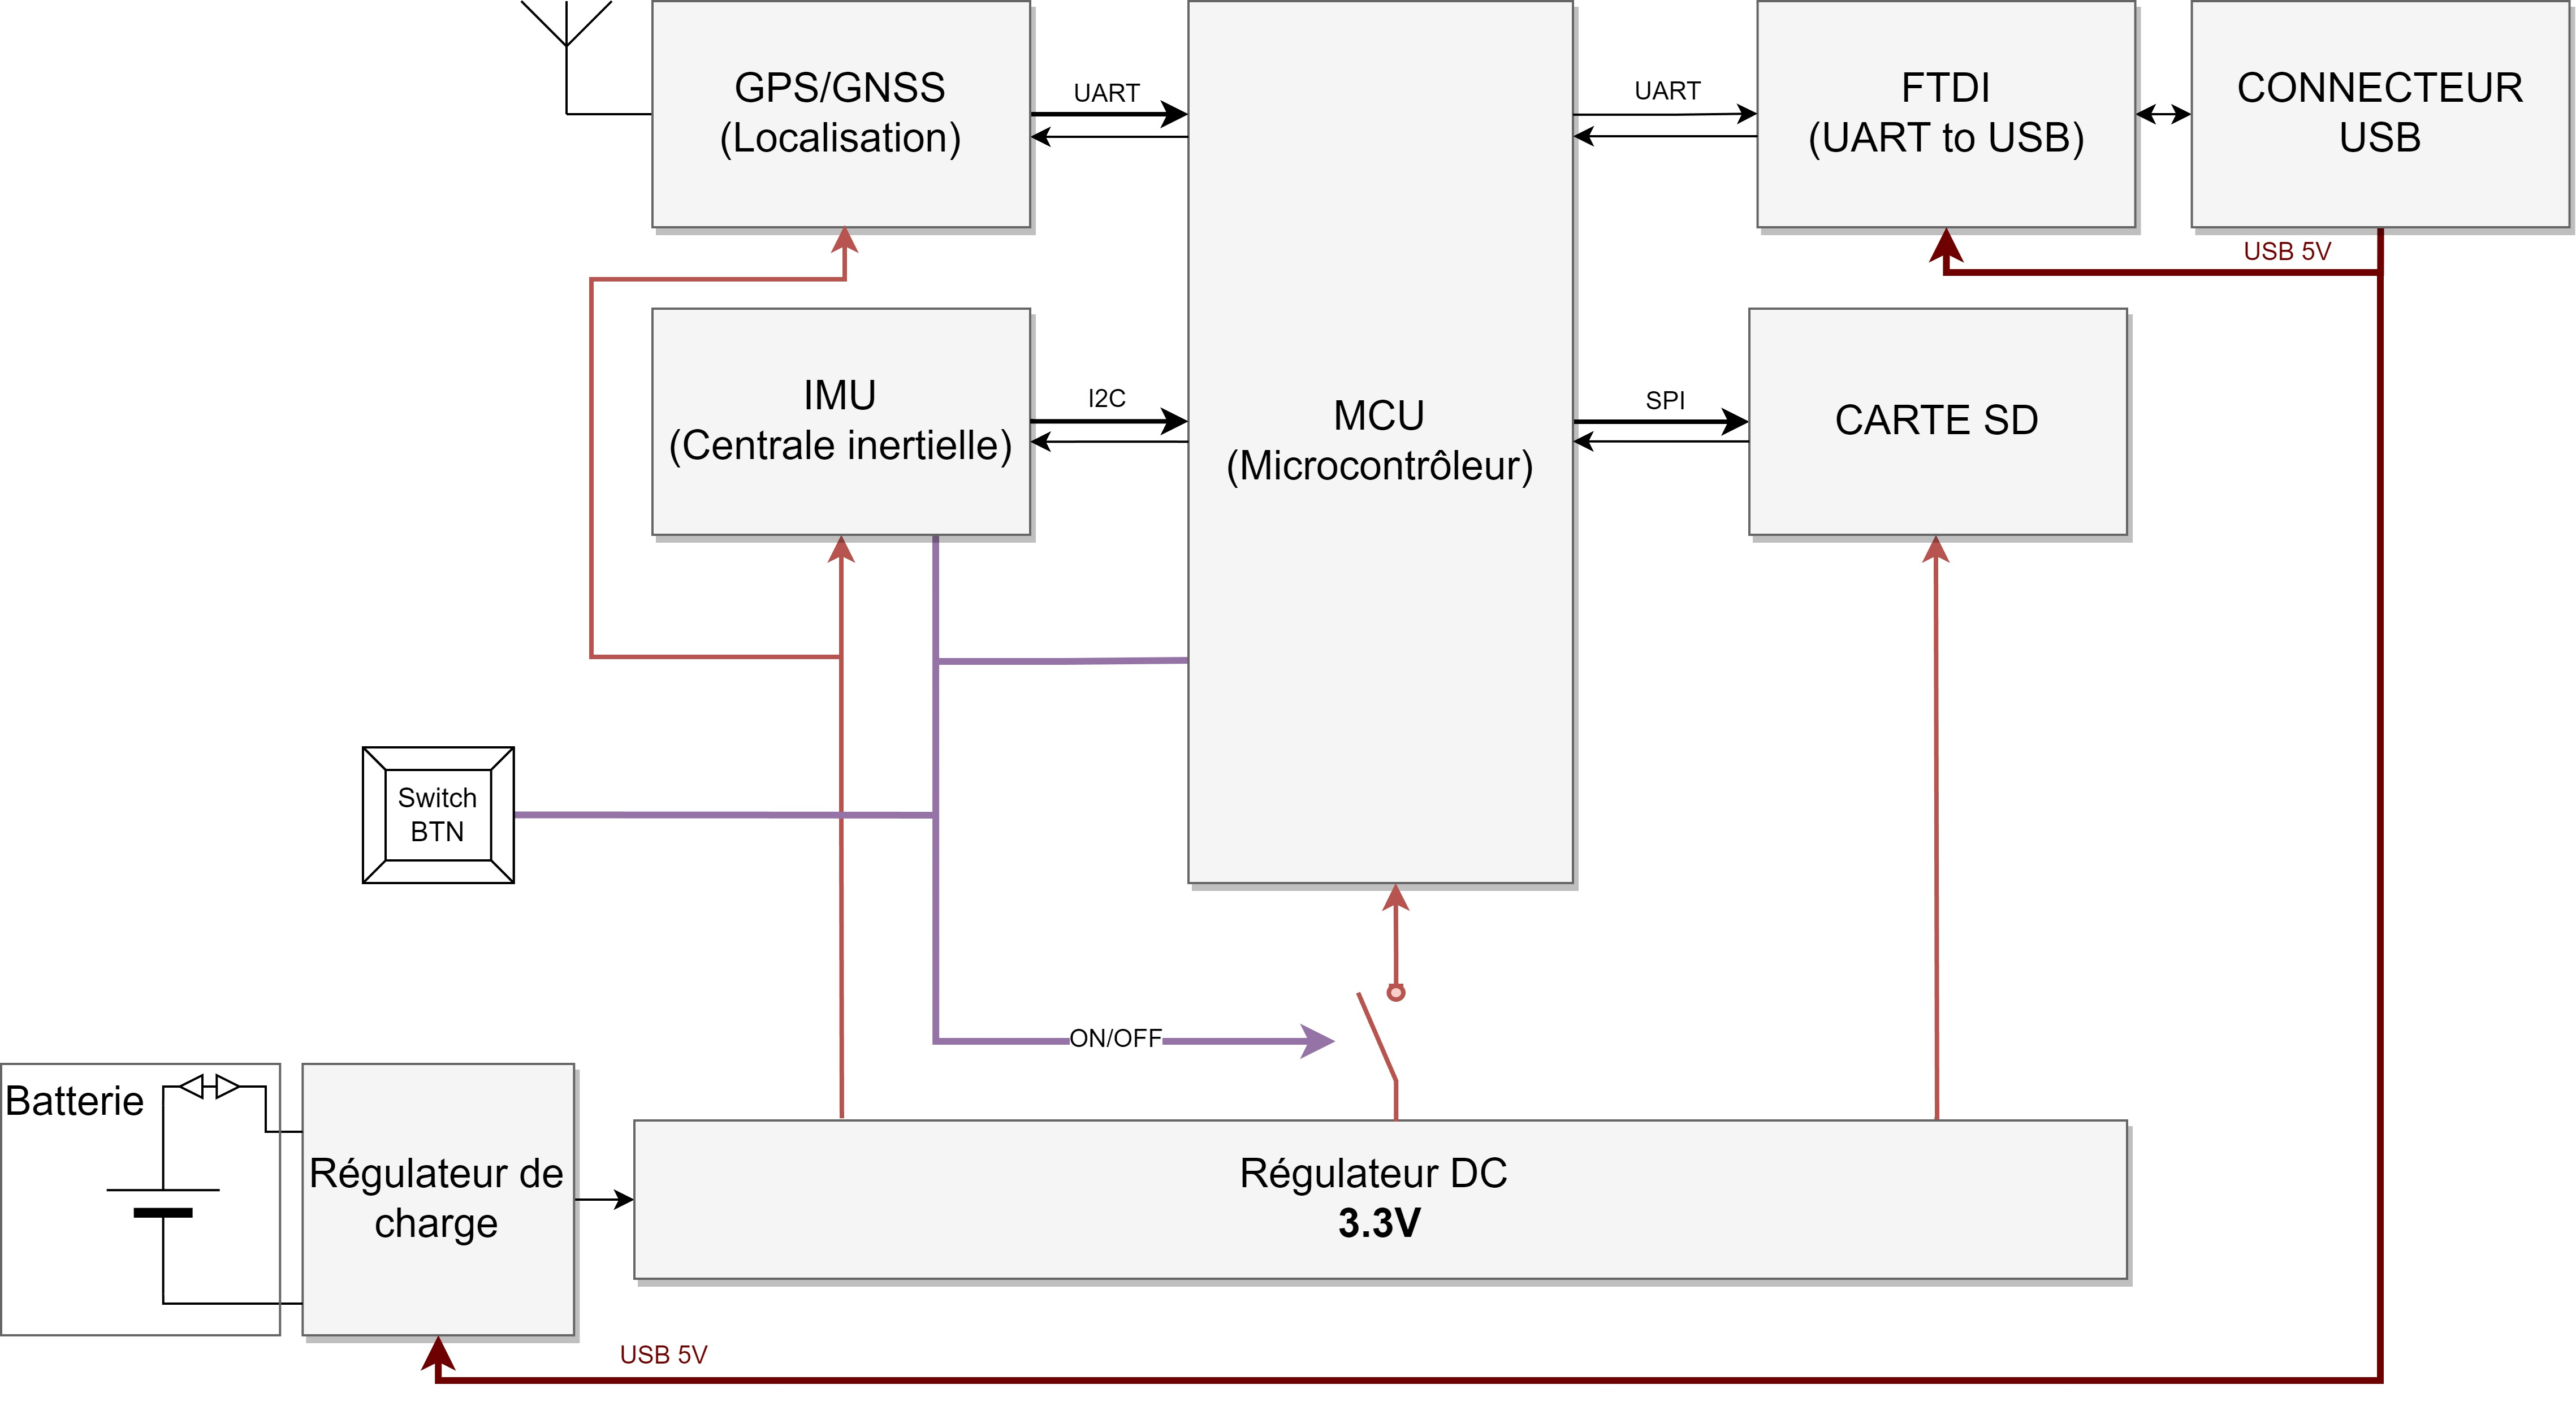
\includegraphics[width=1\textwidth]{../figures/cdc/blocs_grossiers_no_antenna.jpg}
	\caption{Schéma de principe}
	\label{fig:blocsgrossiers}
	\source{Auteur}
\end{figure}


% ---- Description des blocs ----
\subsection{Description des blocs}

\begin{table}[h]
	\resizebox{\columnwidth}{!}{%
		\begin{tabular}{|l|l|}
			\hline
			Bloc        & Description                                     \\ \hline
			\Gls{gnss}. & Récepteur \Gls{rf} avec antenne interne/externe et communication UART. \\ \hline
			\Gls{mcu}.  & Microcontrôleur PIC32, intelligence du système, basse consommation.    \\ \hline
			\Gls{imu}.  & Centrale inertielle, accélération, gyroscope... \\ \hline
			Carte SD    & Stockage des données de vol.                    \\ \hline
			\Gls{FTDI}. & Convertis la communication USB en série.        \\ \hline
			&                                                 \\ \hline
			&                                                 \\ \hline
		\end{tabular}%
	}
\end{table}

\clearpage

% ---- JALONS ----
\subsection{Planification}
\subsubsection{Diagramme de gantt}

\begin{figure}[h]
	\centering
	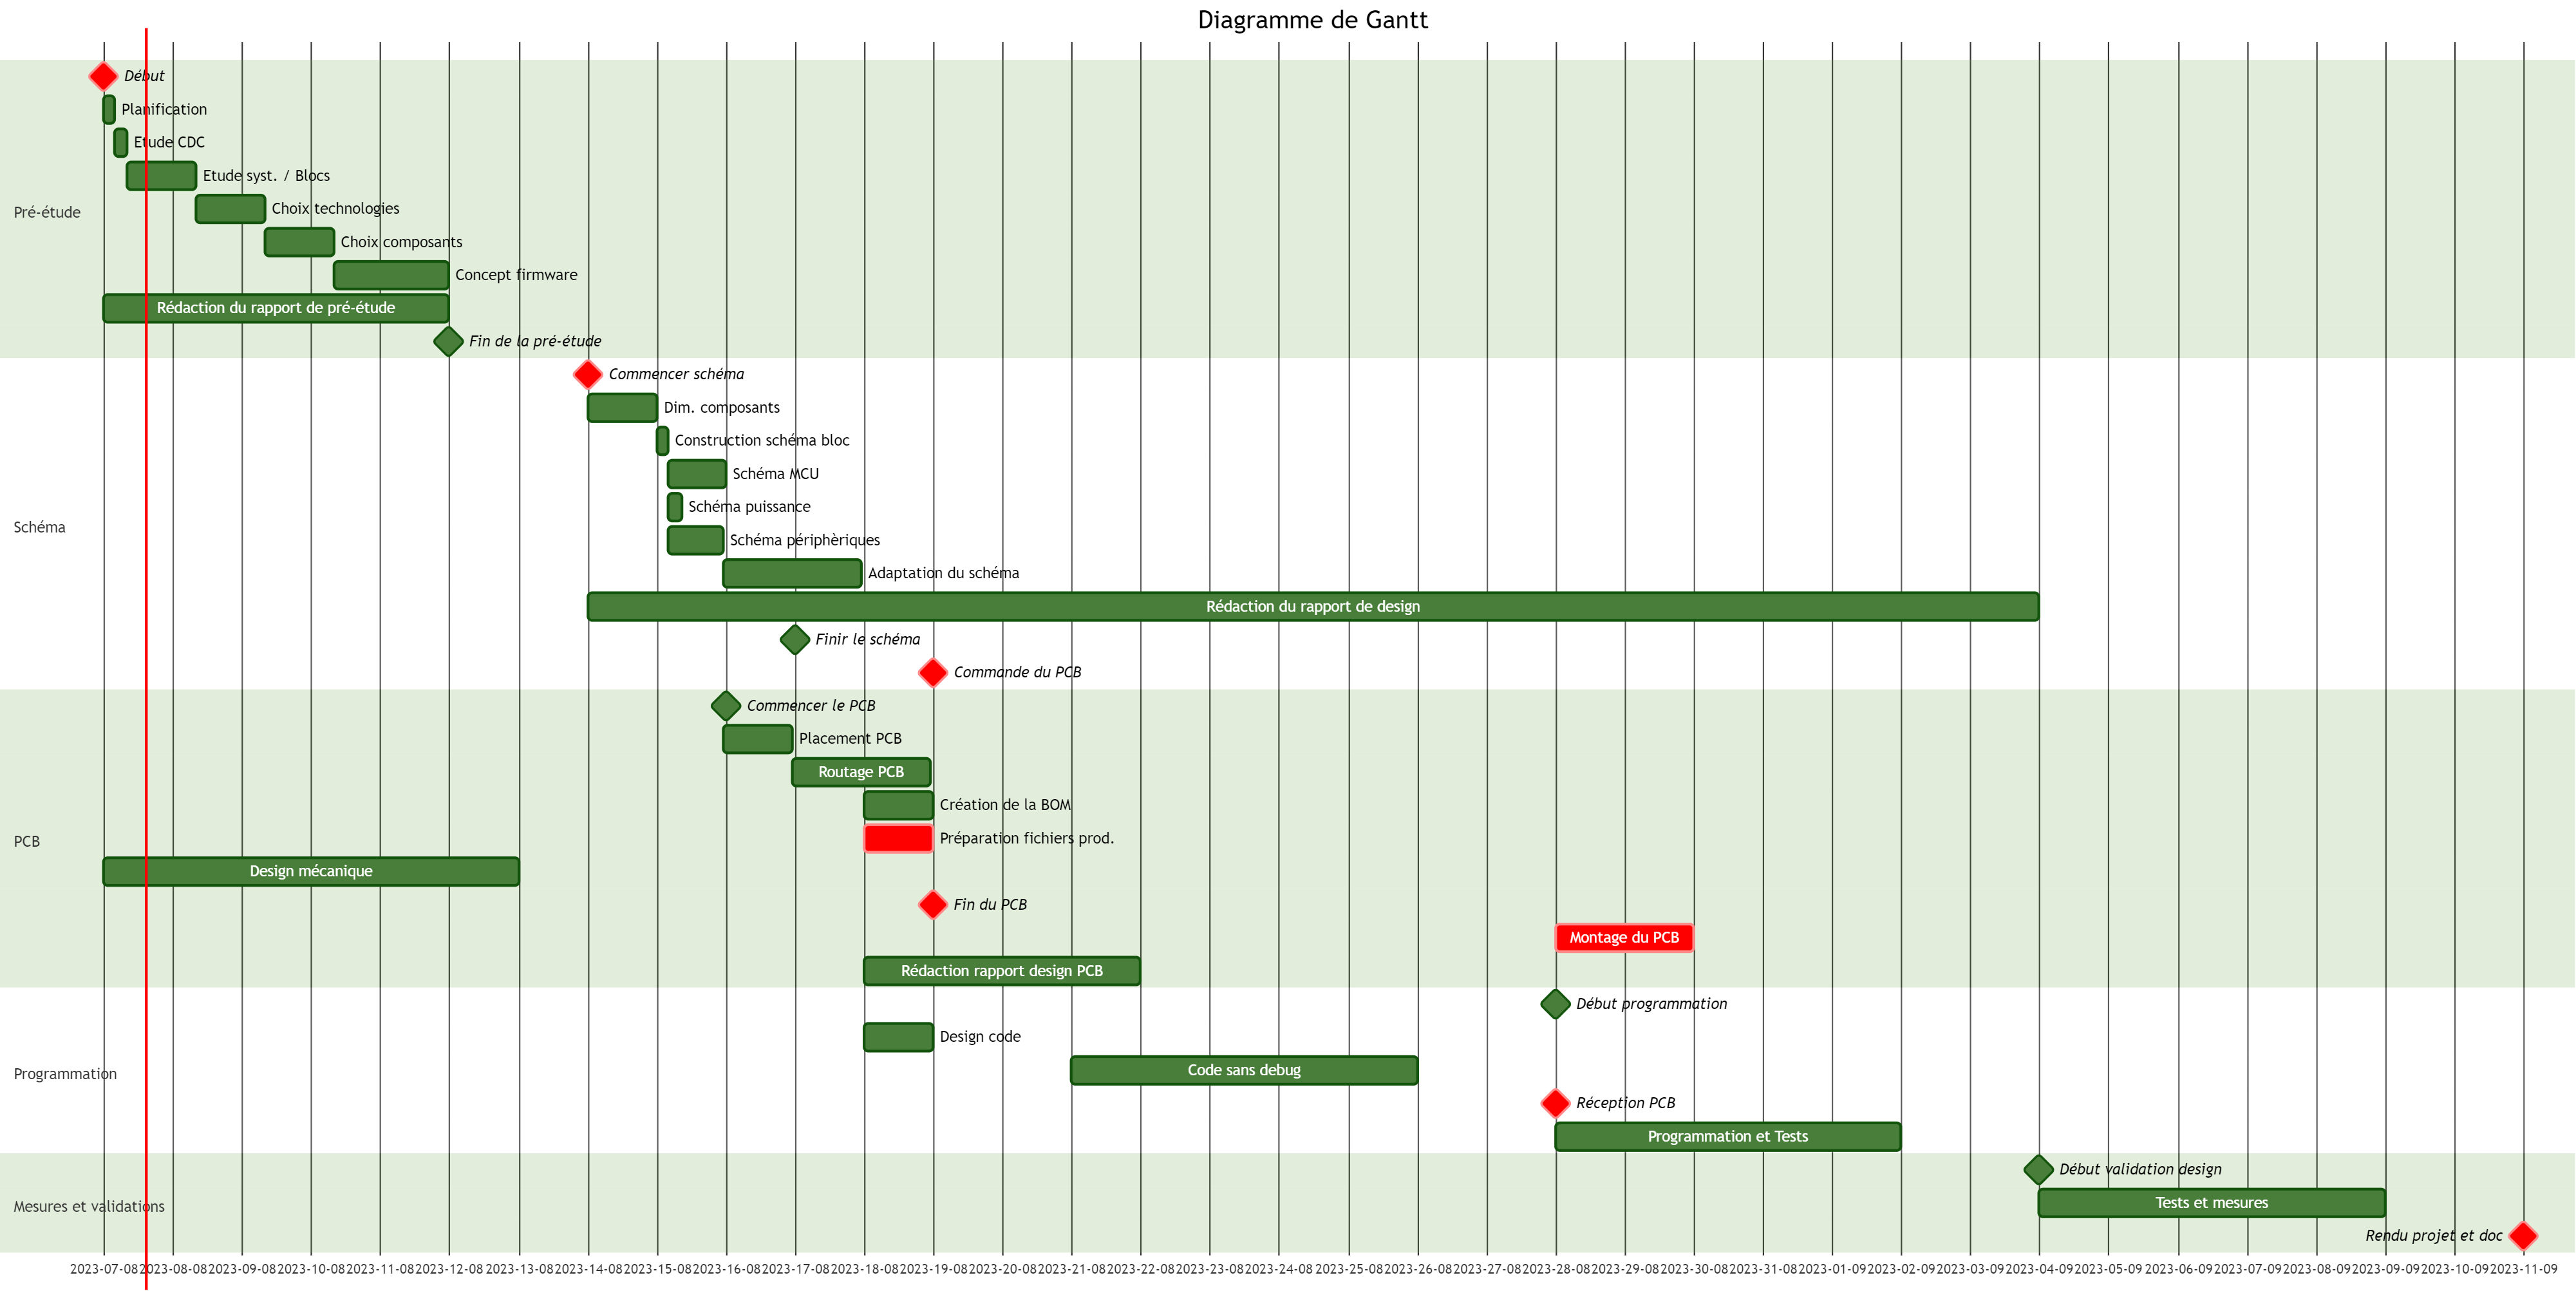
\includegraphics[width=1.1\linewidth]{../figures/cdc/planif}
	\caption{Planification - Diagramme de gantt}
	\source{Auteur}
	\label{fig:planification}
\end{figure}

\subsubsection{Planification théorique}
\begin{figure}[h]
	\centering
	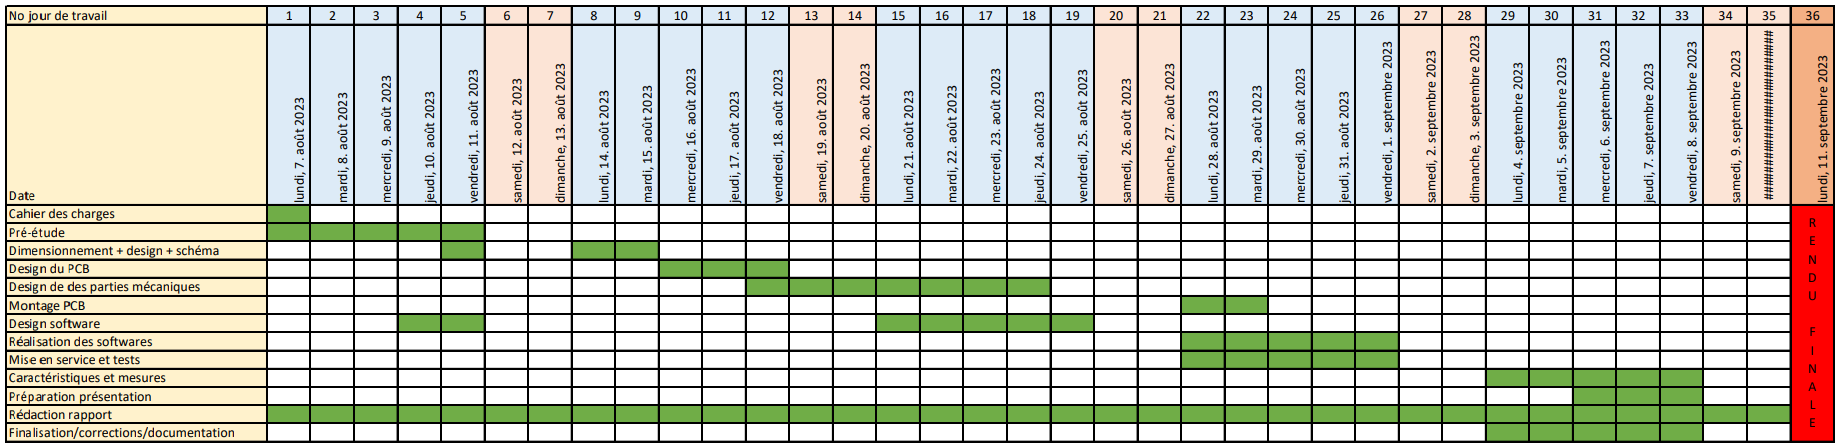
\includegraphics[width=1.1\linewidth]{../figures/cdc/planif_theorique}
	\caption{Planification théorique}
	\label{fig:planiftheorique}
\end{figure}


\subsection{Livrable}
\begin{itemize}
	\item[•] Les fichiers sources de CAO électronique des PCB réalisés
	\item[•] Tout le nécessaire à fabriquer un exemplaire hardware de chaque :
	\item[•] fichiers de fabrication (GERBER) / liste de pièces avec références pour commande / implantation
	\item[•] Prototype fonctionnel
	\item[•] Modifications / dessins mécaniques, etc
	\item[•] Les fichiers sources de programmation microcontrôleur (.c  / .h)
	\item[•] Tout le nécessaire pour programmer les microcontrôleurs (logiciel ou fichier .hex)
	\item[•] Un calcul / estimation des coûts
	\item[•] Un rapport contenant les calculs - dimensionnement de composants - structogramme, etc.
\end{itemize}

\clearpage
